%
% LaTeX report template 
%

% This is a comment: in LaTeX everything that in a line comes
% after a "%" symbol is treated as comment

\documentclass[11pt, a4paper]{article}
\usepackage{graphicx}
\usepackage{amsmath}
\usepackage{listings}
\usepackage{url}

\title{Assignment 3: Fitting Data To Models} % Title of the report

\author{Rohit Kumar [EE20B111]} % Name of Author

\date{\today} % Date for the report
\begin{document}	
		
\maketitle % Insert the title, author and date
\section*{Aim}
%Create new section;it is autonumbered
This assignment is about fitting data to models.\\
The main content of the assignment is: 
\begin{itemize}
\item Analysing data to extract information out of it.
\item To study the effects of noise on the fitting process.
\item To plot a number of different types of graphs. 
\end{itemize}

\section{Extracting, reading and storing the data}
On running the python file \textit{\path{generate_data.py}}, a DAT file \textit{\path{fitting.dat}} is created in the same directory in which the code was compiled. Also, the .py file generates a plot of the function with noises being included.

   \begin{figure}[!tbh]
   	\centering
   	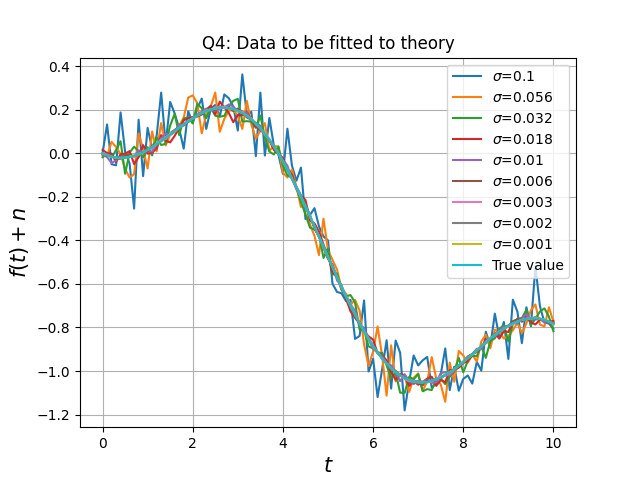
\includegraphics[scale=0.5]{Figure_Q4.png}   
   	\caption{Data plot(Q-4)}
   	\label{fig:sample}
   \end{figure} 
   
   This file(fitting.dat) contains 101 rows with 10 columns of data. The first column is the time values and then the next nine columns are the noisy values of the function as shown below. The standard deviation of each column of the data is given by the python command below:
\begin{verbatim}	
stdev = logspace(-1,-3,9)
\end{verbatim}
\section{Plotting the true and noise added plots}
Since, the actual function is known, we can plot it's graph also. The function is defined in python \textit{\path{EE20B111_Assignment.py}} as the following code snippet:
\begin{verbatim}	
def g(t, A, B):
    return A*sp.jv(2,t) + B*t
\end{verbatim}

On plotting the function's true value along with all the 9 noise added to the true function's values, the following plot was generated. This is the Figure 0 that was asked in Q-3 and Q-4. The python code snippet for plotting the follwing graph is as follows:

\begin{verbatim}	
for i in range(col - 1):
    # Define our legend
    plot(data[:,0],data[:,i+1],label='$\sigma$'+"="+str(np.around(std_dev[i],3))) 
    plt.legend()
\end{verbatim}

	\begin{figure}[!tbh]
   	\centering
   	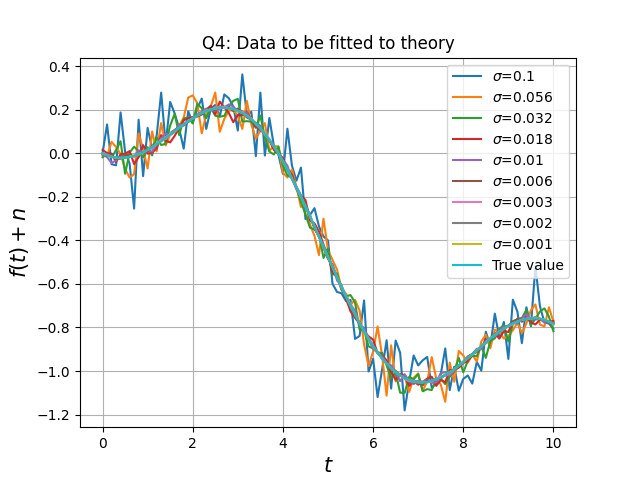
\includegraphics[scale=0.6]{Figure_Q4.png}   
   	\caption{True and noise added plots}
   	\label{fig:sample}
   \end{figure} 
   
\section{The Error plot}
Error bars is a better way of presenting the uncertainty in the reported measurement. The errorbars for the first data column are plotted using the \textbf{errorbar()} function. The python code snippet for plotting the errorbar plot is as follows:
\begin{verbatim}	
plot(t, g(t, 1.05, -0.105), label = r"True value")
errorbar(t[::5], data[::5, 1], std_dev[1], fmt='ro', label = r"Error bar") 
\end{verbatim}
 The graph obtained by plotting every 5th data point with errorbars and the original data is as follows:   
	\begin{figure}[!tbh]
   	\centering
   	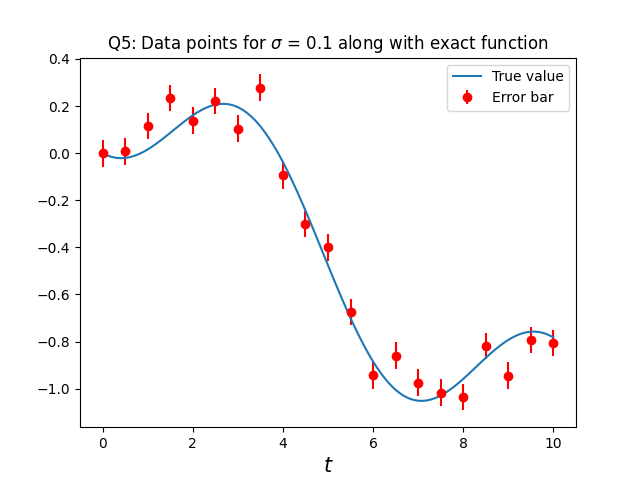
\includegraphics[scale=0.6]{Figure_Q5.png}   
   	\caption{Errorbar plot}
   	\label{fig:sample}
   \end{figure} 
  
\section{The Matrix equation}
The true value function can be created using a matrix equation also. The matrix M when multiplied with (A,B) matrix will give rise to the actual function. This can also be verified by substituting $A=1.05$ and $B=-0.105$. In order to compare 2 matrices, we create a function \path{ismatrix_equal(matA,matB)} whose code snippet is given below:
  \begin{verbatim}	
def ismatrix_equal(matA, matB):
    count = 0 # count is a temporary variable used to store the no. of elements
    
    for i in range(0, row): # Running through all rows
        if matA[i] == matB[i]: # If the element matches                       
            count += 1 # Increment count

    if count == row: # If all elements matched
        return True # Return true
    else: # Else, return false
        return False

if ismatrix_equal(Q, temp):
    print("Both the matrices(Q = MP and g(t, A0, B0)) are equal.")
else: 
    print("Both the matrices(Q = MP and g(t, A0, B0)) are not equal.")           
\end{verbatim} 


\section{The Mean Squared Error}
The mean squared error is the error between the noisy data and the true functional data. It is found out as follows:
$$\varepsilon_{ij} = (\frac{1}{101})\sum_{k=0}^{101}(f_{k} - g(t_{k},A_{i},B_{j}))^{2}$$
The python code snippet to calculate the mean squared error is as follows:
\begin{verbatim}	
epsilon = np.zeros((len(A), len(B)))
for i in range(len(A)):
    for j in range((len(B))):
        epsilon[i,j] = np.mean(np.square(temp - g(t, A[i], B[j])))
\end{verbatim}
The contour plot for $\varepsilon$ for different values of A and B is:
	\begin{figure}[!tbh]
   	\centering
   	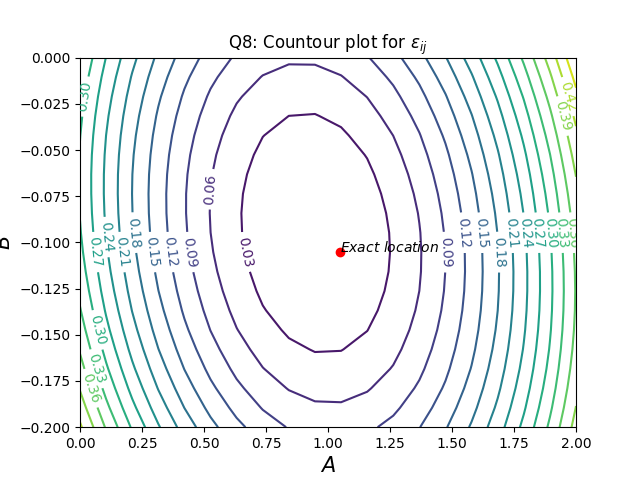
\includegraphics[scale=0.5]{Figure_Q8.png}   
   	\caption{Contour plot}
   	\label{fig:sample}
   \end{figure} 
     
\subsection*{Conclusion}
From the above plot, we can conclude that there exist one and only one minimum for $\varepsilon$.

\section{Error Computation in estimation of A and B} 
It is possible to try and compute the best measure for A and B from the matrix M by using the \textit{lstsq()} function form \textit{scipiy.linalg}.
Using this we can calculate the error in the values of A and B. The python code snippet is as follows:
\begin{verbatim}	
pred = [] # Initialising the required variables
Aerror = []
Berror = []
y_true = g(t, 1.05, -0.105) # True graph 
for i in range(col - 1):
    p, resid, rank, sig = lstsq(M, data[:, i + 1])
    aerr = np.square(p[0] - 1.05) # Auxiliary variable to hold error in A 
    ber = np.square(p[1] + 0.105) # Auxiliary variable to hold error in B
    Aerror.append(aerr) # Updating the error in A
    Berror.append(ber) # Updating the error in B
\end{verbatim}

The plot of the error in A and B against the noise standard deviation is:
	\begin{figure}[!tbh]
   	\centering
   	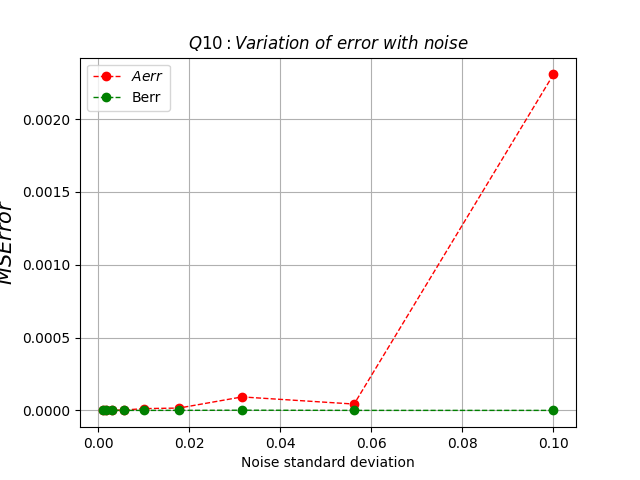
\includegraphics[scale=0.6]{Figure_Q10.png}   
   	\caption{Error vs Standard deviation}
   	\label{fig:sample}
   \end{figure} 

We can also plot the same graph in log scale too. This plot is shown below:\\
 	\begin{figure}[!tbh]
   	\centering
   	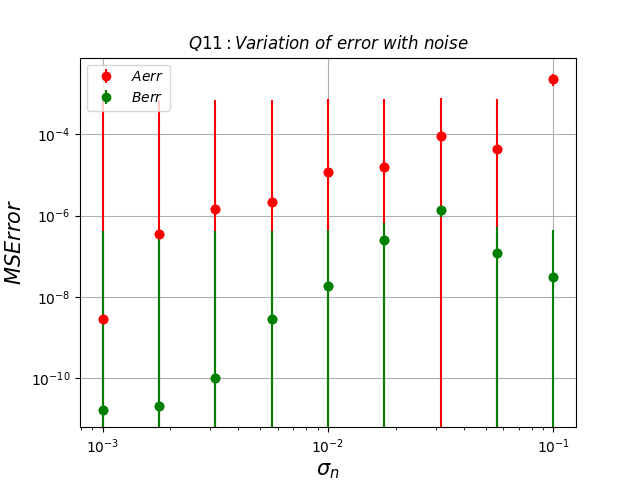
\includegraphics[scale=0.6]{Figure_Q11.png}   
   	\caption{Error vs Standard deviation: log scale}
   	\label{fig:sample}
   \end{figure} 
\subsection*{Conclusion}
From Figure 5, it is evident that the plot is not linear. Also from Figure 6, it is made sure that the plot is not linear in the logscale case too. Hence, in both the cases, the graph is non-linear i.e., the plot is not varying linearly with noise. 

\section*{Inference}
The given noisy data was extracted and the best possible estimate for the
underlying model parameters were found by minimizing the mean squared
error. This is one of the most general engineering use of a computer, modelling of real data.The method of least squares assumes that the best fit curve of a given type is the curve that has the minimal sum of deviations, i.e., least square error from a given set of data. It reduces the error and gives the best fitting data.
 
\end{document}
